\section{Muhammad Dzihan Al-Banna(1174095)}
\subsection{PYSHP Reader}
\begin{enumerate}
    \item Buatlah Script Python dan jelaskan berbaris
    \lstinputlisting[firstline=1, lastline=4]{src/1174095/3/praktek2.py}
    \hfill\break
    \begin{figure}[H]
		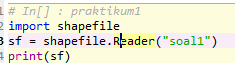
\includegraphics[width=4cm]{figures/1174095/3/1.png}
		\centering
		\caption{Hasil SHP Reader Soal 1}
    \end{figure}
    
    \item Buatlah Script Python dan jelaskan berbaris
    \lstinputlisting[firstline=6, lastline=8]{src/1174095/3/praktek2.py}
    \hfill\break
    \begin{figure}[H]
		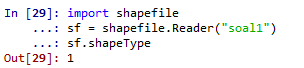
\includegraphics[width=4cm]{figures/1174095/3/2.png}
		\centering
		\caption{Hasil SHP Reader Soal 2}
    \end{figure}
    
    \item Buatlah Script Python dan jelaskan berbaris
    \lstinputlisting[firstline=10, lastline=12]{src/1174095/3/praktek2.py}
    \hfill\break
    \begin{figure}[H]
		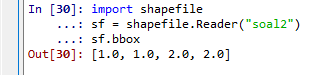
\includegraphics[width=4cm]{figures/1174095/3/3.png}
		\centering
		\caption{Hasil SHP Reader Soal 3}
    \end{figure}
    
    \item Buatlah Script Python dan jelaskan berbaris
    \lstinputlisting[firstline=14, lastline=17]{src/1174095/3/praktek2.py}
    \hfill\break
    \begin{figure}[H]
		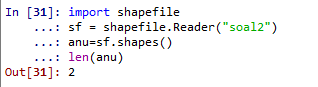
\includegraphics[width=4cm]{figures/1174095/3/4.png}
		\centering
		\caption{Hasil SHP Reader Soal 4}
    \end{figure}
    
    \item Buatlah Script Python dan jelaskan berbaris
    \lstinputlisting[firstline=19, lastline=23]{src/1174095/3/praktek2.py}
    \hfill\break
    \begin{figure}[H]
		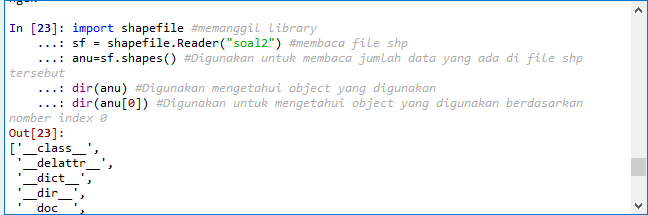
\includegraphics[width=4cm]{figures/1174095/3/51.png}
		\centering
		\caption{Hasil SHP Reader Soal 5 Codingan}
    \end{figure}

    \hfill\break
    \begin{figure}[H]
		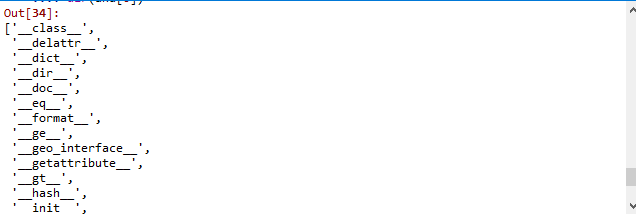
\includegraphics[width=4cm]{figures/1174095/3/5.png}
		\centering
		\caption{Hasil SHP Reader Soal 5 Hasil}
    \end{figure}
    
    \item Buatlah Script Python dan jelaskan berbaris
    \lstinputlisting[firstline=25, lastline=28]{src/1174095/3/praktek2.py}
    \hfill\break
    \begin{figure}[H]
		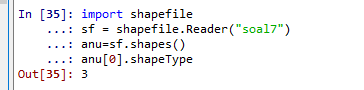
\includegraphics[width=4cm]{figures/1174095/3/6.png}
		\centering
		\caption{Hasil SHP Reader Soal 6}
    \end{figure}

    \item Buatlah Script Python dan jelaskan berbaris
    \lstinputlisting[firstline=30, lastline=34]{src/1174095/3/praktek2.py}
    \hfill\break
    \begin{figure}[H]
		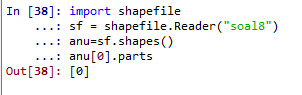
\includegraphics[width=4cm]{figures/1174095/3/7.png}
		\centering
		\caption{Hasil SHP Reader Soal 7}
    \end{figure}

    \item Buatlah Script Python dan jelaskan berbaris
    \lstinputlisting[firstline=36, lastline=39]{src/1174095/3/praktek2.py}
    \hfill\break
    \begin{figure}[H]
		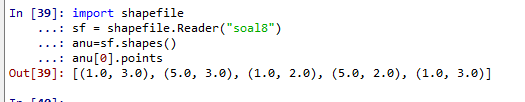
\includegraphics[width=4cm]{figures/1174095/3/8.png}
		\centering
		\caption{Hasil SHP Reader Soal 8}
    \end{figure}

    \item Buatlah Script Python dan jelaskan berbaris
    \lstinputlisting[firstline=41, lastline=44]{src/1174095/3/praktek2.py}
    \hfill\break
    \begin{figure}[H]
		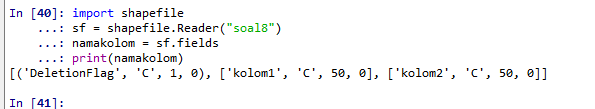
\includegraphics[width=4cm]{figures/1174095/3/9.png}
		\centering
		\caption{Hasil SHP Reader Soal 9}
    \end{figure}

    \item Buatlah Script Python dan jelaskan berbaris
    \lstinputlisting[firstline=46, lastline=49]{src/1174095/3/praktek2.py}
    \hfill\break
    \begin{figure}[H]
		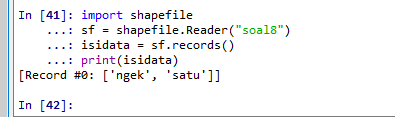
\includegraphics[width=4cm]{figures/1174095/3/10.png}
		\centering
		\caption{Hasil SHP Reader Soal 10}
    \end{figure}

     \item Buatlah Script Python dan jelaskan berbaris
    \item \lstinputlisting[firstline=52, lastline=56]{src/1174027/3/praktikum2.py}
    \hfill\break
    \begin{figure}[H]
		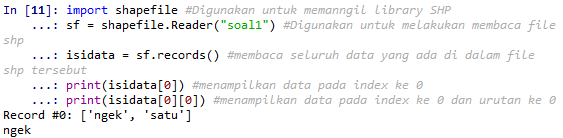
\includegraphics[width=4cm]{figures/1174027/3/soal11.png}
		\centering
		\caption{Hasil SHP Reader Soal 11}
    \end{figure}
\end{enumerate}
\subsection{Link Youtube}
\href{https://youtu.be/ZcSSTLyMdXE}{Video Youtube}